\documentclass{article}
\usepackage{amsmath,amssymb,amsthm,latexsym,paralist,url}
\usepackage[margin=1in]{geometry}
\usepackage{tikz}
\usetikzlibrary{arrows,automata}
\usepackage{csquotes}

\theoremstyle{definition}
\newtheorem{problem}{Problem}
\newtheorem*{solution}{Solution}
\newtheorem*{resources}{Resources}


\newcommand{\honor}{\noindent \textbf{Aggie Honor Statement: }On my honor as an Aggie, I have neither
  given nor received any unauthorized aid on any portion of the academic work included in this assignment.
}

 
\newcommand{\checklist}{\noindent\textbf{Checklist:}
Did you...
\begin{compactenum}
\item abide by the Aggie Honor Code?
\item solve all problems?
\item start a new page for each problem?
\item show your work clearly?
\item type your solution?
\item submit a PDF to gradescope?
\end{compactenum}
}

\newcommand{\problemset}[1]{\begin{center}\textbf{Homework #1}\end{center}}
\newcommand{\duedate}[1]{\begin{quote}\textbf{Due: #1} on gradescope (\url{gradescope.com}). \\You must show your work in order to receive credit.\end{quote}}

%%% CONSTANTS
\newcommand{\mysemester}[0]{Spring 2018}
\newcommand{\mysectionnumber}[0]{501,502}
\newcommand{\myname}[0]{Hunter Cleary}
\newcommand{\homeworknumber}[0]{5}

%%% HEADERS & FOOTERS
\usepackage{fancyhdr} % This should be set AFTER setting up the page geometry
\pagestyle{fancy} % options: empty , plain , fancy
\renewcommand{\headrulewidth}{0pt} % customise the layout...
\lhead{CSCE 222-\mysectionnumber}\chead{Homework \homeworknumber}\rhead{\myname}
\lfoot{}\cfoot{\thepage}\rfoot{}

\title{CSCE 222: Discrete Structures for Computing\\Section \mysectionnumber\\\mysemester}
\author{\myname}
\date{}

\begin{document}

\maketitle
\problemset{\homeworknumber}
\duedate{25 February 2017 (Sunday) before 11:59 p.m.}
\bigskip

\honor
\bigskip

\checklist

% Sets
\begin{problem} (25 points)\\
Use set builder notation to give a description of each set.
\begin{compactenum}
\item $\{0,2,4,6,8,10\}$
\item $\{-9,-6,-3,0,3,6,9\}$
\item $\{s,p,q,r\}$
\item $\{0,1,4,9,16,25,36,49,64,81\}$
\end{compactenum}
\end{problem}

\begin{solution}\ \\
\begin{compactenum}
\item $\{2n \|n \in \mathbb{N} , 0 \leq n \leq 5 \}$\ \\
\item $\{3n \|n \in \mathbb{Z} , -3 \leq n \leq 3 \}$\ \\
\item $\{x \| $ x is an alphabet $,s \leq x \leq r \}$\ \\
\item $\{n^2 \| n \in \mathbb{N} , 0 \leq x \leq 9\}$\ \\
\end{compactenum}
\end{solution}

\newpage

% Sets
\begin{problem}(25 points)\\ 
Use a single Venn diagram to illustrate the relationship $A \subset B$ and $A \subset C$.\\
\textit{Your diagram must be exactly and unambiguously "$A \subset B$ and $A \subset C$".}
\end{problem}

\begin{solution}\ \\
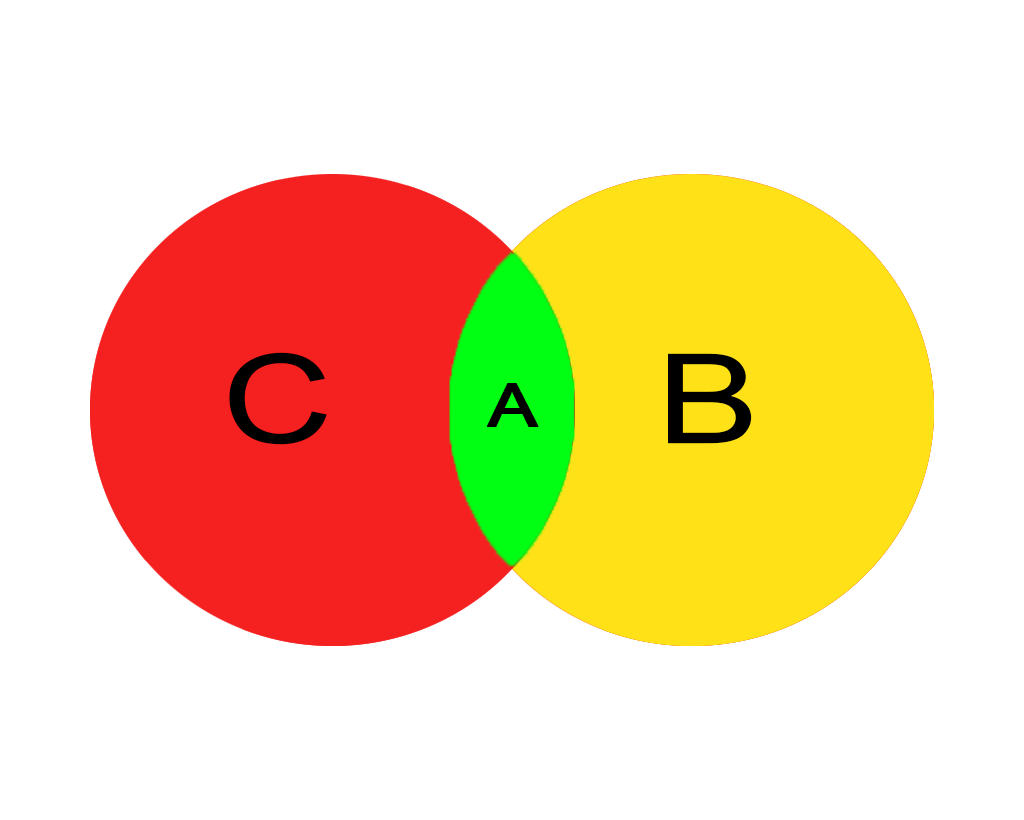
\includegraphics[width=\textwidth,height=\textheight,keepaspectratio]{Venn1.png}
\end{solution}

\newpage

% Set Operations
\begin{problem} (25 points)\\
Determine whether symmetric difference is associative: that is, if $A, B$, $C$ are sets, does it follow that $A\oplus(B\oplus C) = (A\oplus B) \oplus C$?\\
\textit{Justify your answer in two ways: Venn diagrams, logical proof involving set identities.}
\end{problem}

\begin{solution}\ \\
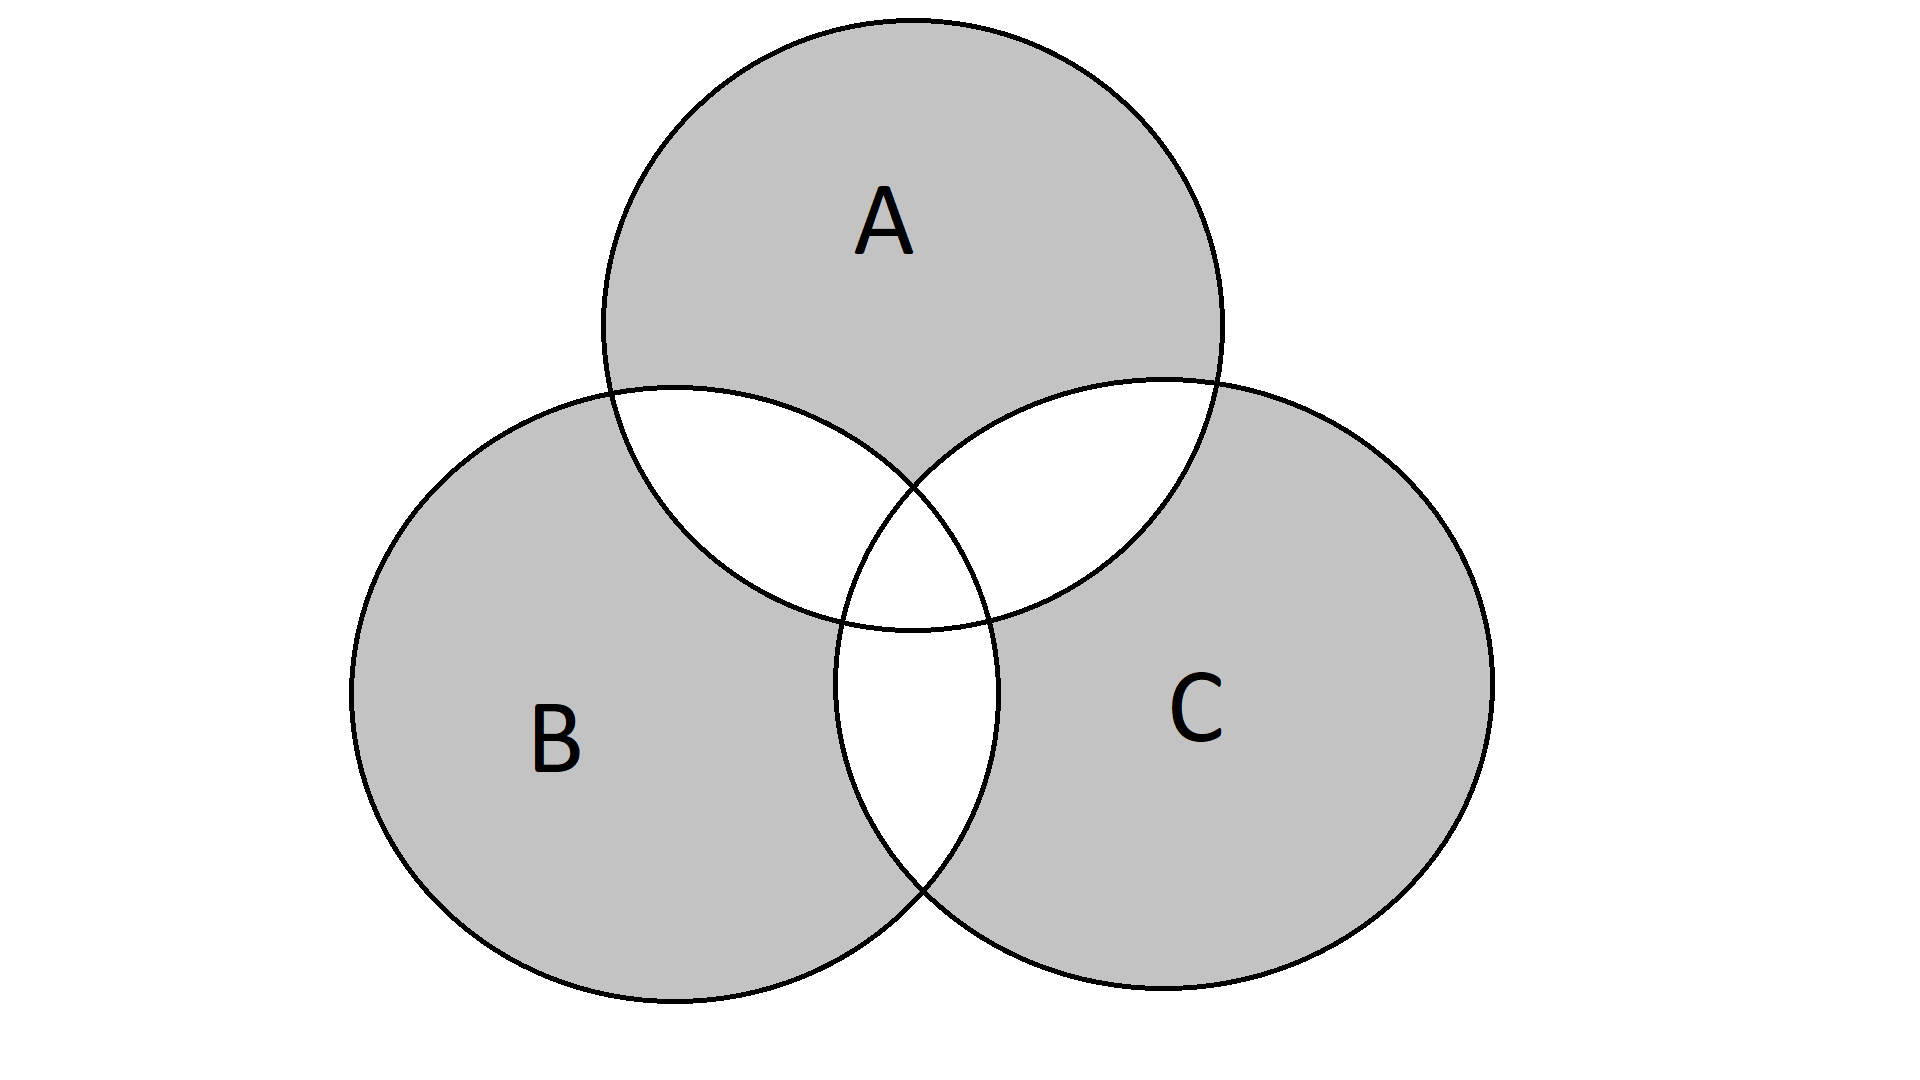
\includegraphics[width=\textwidth,height=\textheight,keepaspectratio]{Venn2.png}\ \\
$A\oplus(B\oplus C) = (A\oplus B) \oplus C$\ \\ \ \\
$A\oplus(B\oplus C)$\ \\
$\equiv A\vee(B\oplus C) \wedge \neg(A \wedge (B \oplus C))$\ \\
$\equiv A\vee((B \vee C) \wedge \neg(B \wedge C)) \wedge \neg(A \wedge ((B \vee C) \wedge \neg(B \wedge C))$\ \\ \ \\ 
$(A\oplus B) \oplus C$$\ \\
$\equiv (C \vee (A \oplus B) \wedge \neg(C \wedge (A\oplus B))$\ \\
$\equiv (C \vee ((A \vee B) \wedge \neg (A \wedge B)) \wedge \neg(C \wedge (A \vee B) \wedge \neg (A \wedge B))$\ \\
$\equiv A\vee((B \vee C) \wedge \neg(B \wedge C)) \wedge \neg(A \wedge ((B \vee C) \wedge \neg(B \wedge C))$\ \\


\end{solution}

\newpage

% Set Operations
\begin{problem}(25 points)\\
Prove the 3-set case of the principle of inclusion-exclusion: if $A, B$, and $C$ are sets, then
\begin{align*}
|A\cup B \cup C| = &|A| + |B| + |C|\\
&-|A \cap B| - |A \cap C| - |B \cap C|\\
&+|A \cap B \cap C|
\end{align*}
\textit{Hint: use the 2-set case of the principle of inclusion exclusion.}
\end{problem}

\begin{solution}\ \\
\begin{compactenum}
The inclusion exclusion principle is an equation relating to two sets and their union. If A and B are two finite sets then: 
$|A \cup B| = |A| + |B| - |A \cap B|$.
This is equivalent to saying that the union of two finite sets is equal to the sum of the two sets minus one set of the elements that the two share in common.\ \\
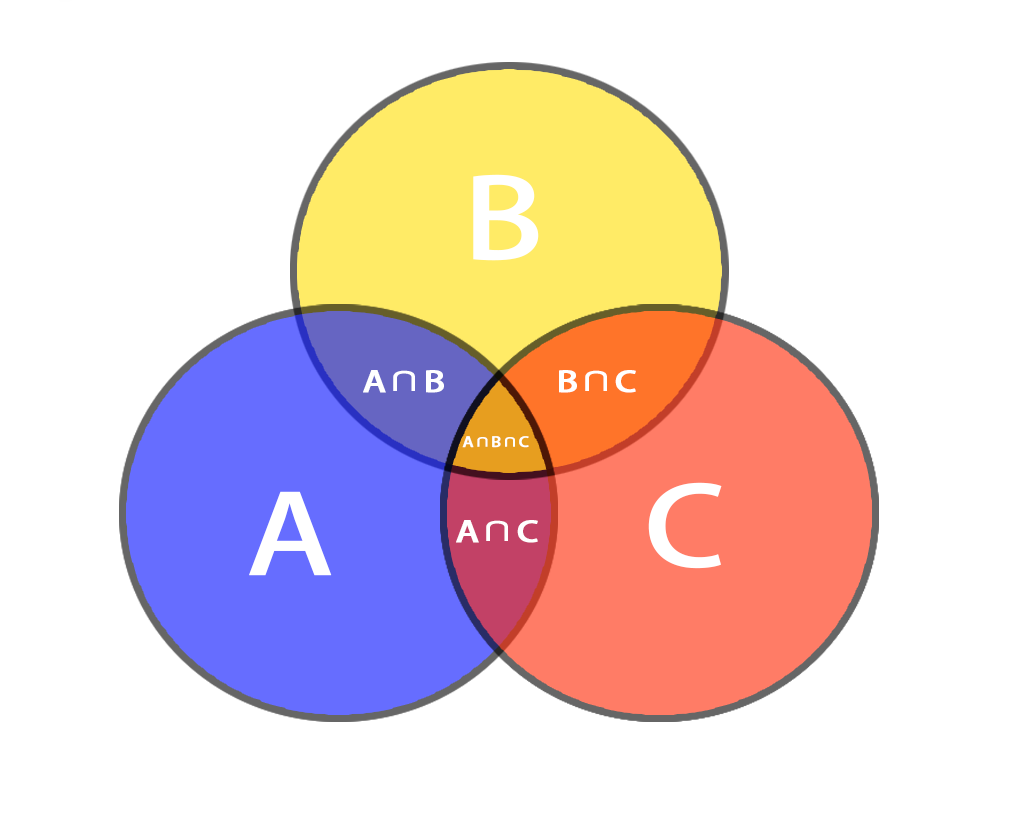
\includegraphics[width=\textwidth,height=\textheight,keepaspectratio]{Venn3.png}

$|A \cup B| = |A| + |B| - |A \cap B|$\ \\ 
$|B \cup C| = |B| + |C| - |B \cap C|$\ \\
$|C \cup A| = |A| + |C| - |A \cap C|$\ \\
$\therefore |A\cup B \cup C| = &|A| + |B| + |C|
-|A \cap B| - |A \cap C| - |B \cap C| +|A \cap B \cap C|$

\end{compactenum}
\end{solution}

\newpage

\end{document}
